\chapter{The Eigenvalue Eigenvector Problem}
In this chapter we look at the important eigenvalue-eigenvector question.  In this
question we wish to find vectors $\bx$ and values $\lambda$ such that $A \bx = \lambda
\bx$ for some given square matrix $A$.  This has profound impact on how we understand
differential equations but it also have profound impact on how we understand bases, matrix
multiplication, and many other important aspects of linear algebra.  Furthermore, we can
extend the idea to linear operators and view certain linear differential equations as eigenvalue
questions.  Wow \ldots just wow \ldots you're going to love this chapter!

\section{Introduction To Eigenvalues}
\begin{definition}[The Eigenvalues and Eigenvectors of a Matrix]
    Let $A$ be a square $n\times n$ matrix.  In the equation $A \bx = \lambda \bx$, the
    vector $\bx \in \mathbb{R}^n$ is called an eigenvector of the matrix $A$ and $\lambda$
    is the associated eigenvalue.
\end{definition}

\begin{problem}
    In the applet 
        \href{http://www.geogebra.org/m/334841}{http://www.geogebra.org/m/334841}
    you will find a way to graphically manipulate vectors to approximate eigenvectors in
    $\mathbb{R}^2$.  Use the applet to approximate the eigenvectors and eigenvalues of $A
    = \begin{pmatrix} 0 & 2 \\ 1 & -1 \end{pmatrix}$.
\end{problem}
\solution{
Eigenvectors are $(2,1)^T$ and $(-1,1)^T$ with eigenvalues $1$ and $-2$ respectively.
}


\begin{problem}
    Which of the following is an eigenvector of the matrix \( \left( \begin{array}{cc} 2 &
        -1 \\ -4 & -1 \end{array} \right) \)?
\begin{enumerate}
    \item[(a)] \( \left( \begin{array}{c} 4 \\ 1 \end{array} \right) \)
    \item[(b)] \( \left( \begin{array}{c} -1 \\ 4 \end{array} \right) \)
    \item[(c)] \( \left( \begin{array}{c} 1 \\ 4 \end{array} \right) \)
    \item[(d)] \( \left( \begin{array}{c} 1 \\ -4 \end{array} \right) \)
    \item[(e)] None of the above
    \item[(f)] More than one of the above
\end{enumerate}
\end{problem}
% \begin{problem}
%     \begin{itemize}
%             \input{ClickerQuestions/LA.00.11.130}
%     \end{itemize}
% \end{problem}
\solution{
    The vector $\begin{pmatrix} 1 \\ 4 \end{pmatrix}$ is the only eigenvector and it has
    eigenvalue $\lambda = -2$.
}

\begin{problem}
    Suppose the matrix $A = \left( \begin{array}{cc} a & b \\ c & d \end{array} \right) $
    has an eigenvalue 1 with associated eigenvector $x = \left( \begin{array}{c} 2 \\ 3
    \end{array} \right).$ What is $A^{50}x$?
\begin{enumerate}
    \item[(a)] $\left( \begin{array}{cc}
a & b \\
c & d
\end{array} \right) $ 
\item[(b)] $\left( \begin{array}{cc}
a^{50} & b^{50} \\
c^{50} & d^{50}
\end{array} \right) $ 
\item[(c)] $\left( \begin{array}{c} 2 \\ 3 \end{array} \right)$
\item[(d)] $\left( \begin{array}{c} 2^{50} \\ 3^{50} \end{array} \right)$
\item[(e)] Way too hard to compute.
\end{enumerate}
\end{problem}
% \begin{problem}
%     \begin{itemize}
%             \input{ClickerQuestions/LA.00.11.150}
%     \end{itemize}
% \end{problem}
\solution{
choice c
}

\begin{problem}
    Vector $\bx$ is an eigenvector of matrix $A$. If $\bx = \left( \begin{array}{c} 1 \\ 3
    \end{array} \right)$ and $Ax = \left( \begin{array}{c} 4 \\ 12 \end{array}\right)$,
    then what is the associated eigenvalue?
\begin{enumerate}
    \item[(a)] 1
    \item[(b)] 3
    \item[(c)] 4
    \item[(d)] Not enough information is given.
\end{enumerate}
\end{problem}
% \begin{problem}
%     \begin{itemize}
%             \input{ClickerQuestions/LA.00.11.155}
%     \end{itemize}
% \end{problem}
\solution{eigenvalue = 4 (choice c)}

\begin{technique}[Finding Eigenvalues and Eigenvectors]
    To find the eigenvalues of an $n \times n$ matrix $A$:
        \begin{itemize}
            \item Rearrange the equation $A \bx = \lambda \bx$ so that the right-hand side
                is the zero vector: 
                \[ \underline{\hspace{1in}} = \bo \]
            \item Eigenvectors are \underline{never} the zero vector so what does the
                previous equation imply about the matrix $A - \lambda I$?
            \item Form the characteristic polynomial: $p(\lambda) = \det(A-\lambda I)$ and
                solve for $\lambda$ using algebra
            \item Find the associated eigenspace: 
                \[ E_\lambda = \{ \bx \, : \, (A - \lambda I) \bx = \bo \} \]
        \end{itemize}

\end{technique}
\solution{
    \begin{itemize}
        \item $\left( A - \lambda I \right) \bx = \bo$
        \item The matrix $A - \lambda I$ must be singular so the determinant must be
            zero.
    \end{itemize}
}



\begin{problem}
    Find the eigen-pairs for the matrix
    \[ A = \begin{pmatrix} 5 & 7 \\ -2 & -4 \end{pmatrix} \]
\end{problem}
\solution{
    \[ \lambda_1 = -2, \quad \bv_1 = \begin{pmatrix} 1 \\ -1 \end{pmatrix} \qquad
    \lambda_2 = 3, \quad \bv_2 = \begin{pmatrix} 7 \\ -2 \end{pmatrix} \]
}

\begin{problem}
    The matrix $A = \begin{pmatrix} 3 & 2 \\ 4 & 10 \end{pmatrix}$ has eigenvalue
    $\lambda_1 = 2$.  Find the associated eigenspace $E_{\lambda_1}$.  In other words,
    find the space spanned by the associated eigenvector(s).
\end{problem}
\solution{
    Since $\lambda_1 = 2$ is an eigenvalue of $A$ we need to solve the homogeneous system
    $(A - 2I)\bv = \bo$ for $\bv$.  Observe that $A - 2I = \begin{pmatrix} 1 & 2 \\ 4 & 8
    \end{pmatrix}$ and we can row reduce to $A - 2I \to \begin{pmatrix} 1 & 2 \\ 0 & 0
    \end{pmatrix}$.  Therefore
    \[ \bv = \begin{pmatrix} v_1 \\ v_2 \end{pmatrix} = \begin{pmatrix} -2 \\ 1
    \end{pmatrix} \]
    so 
    \[ E_{\lambda_1} = \text{span}\left\{ \begin{pmatrix} -2 \\ 1 \end{pmatrix} \right\}.
    \]
}


\begin{problem}
    For any integer $n$, what will this product be?  \( \left( \begin{array}{cc} 1 & 2 \\
        2 & 1 \end{array} \right)^n   \left( \begin{array}{c} 1 \\ 5 \end{array}
    \right) \)
\begin{enumerate}
    \item[(a)] \( -1   (3)^n \left( \begin{array}{c} 1 \\ 1 \end{array} \right) + 3   (-2)^n \left( \begin{array}{c} 1 \\ -1 \end{array} \right) \)
    \item[(b)] \( 3   (-1)^n \left( \begin{array}{c} 1 \\ 1 \end{array} \right) + (-2)   3^n \left( \begin{array}{c} 1 \\ -1 \end{array} \right) \)
    \item[(c)] \( 3   (3)^n \left( \begin{array}{c} 1 \\ 1 \end{array} \right) + (-2)   (-1)^n \left( \begin{array}{c} 1 \\ -1 \end{array} \right) \)
    \item[(d)] \( 3   (3)^n \left( \begin{array}{c} 1 \\ 1 \end{array} \right) + (-1)   (-2)^n \left( \begin{array}{c} 1 \\ -1 \end{array} \right) \)
    \item[(e)] None of the above
    \item[(f)] More than one of the above
\end{enumerate}
\end{problem}
% \begin{problem}
%     \begin{itemize}
%             \input{ClickerQuestions/LA.00.11.120}
%     \end{itemize}
% \end{problem}



\begin{problem}
    $\left( \begin{array}{c} 4/3 \\ 1 \end{array} \right)$ is an eigenvector of $\left(
    \begin{array}{cc} 2 & 4 \\ 3 & 1 \end{array} \right).$ What is the associated
    eigenvalue? (Think! Don't solve for all the eigenvalues and eigenvectors.)

\begin{enumerate}
    \item[(a)] 4/3
\item[(b)] 5
\item[(c)] -2
\end{enumerate}
\end{problem}
% \begin{problem}
%     \begin{itemize}
%             \input{ClickerQuestions/LA.00.11.170}
%     \end{itemize}
% \end{problem}
\solution{
    The eigenvalue must be $5$ since the product of the matrix and the vector is $5$ times
    the original vector.
}


\begin{problem}
    If a vector $x$ is in the eigenspace of $A$ corresponding to $\lambda$, and $\lambda
    \neq 0$, then $x$ is

\begin{enumerate}
    \item[(a)] in the nullspace of the matrix $A.$
    \item[(b)] in the nullspace of the matrix $A - \lambda I.$
    \item[(c)] not the zero vector.
    \item[(d)] More than one of the above correctly completes the sentence.
\end{enumerate}
\end{problem}
% \begin{problem}
%     \begin{itemize}
%             \input{ClickerQuestions/LA.00.12.010}
%     \end{itemize}
% \end{problem}
\solution{
    2: in the null space of the matrix $A - \lambda I$.
}

\begin{problem}
    Explain why an $n \times n$ matrix can have at most $n$ distinct eigenvalues.
\end{problem}
\solution{
    The characteristic polynomial is $n^{th}$ order and by the fundamental theorem of
    algebra has at most $n$ distinct roots.
}

\begin{example}
    Find the eigenvalues and eigenvectors of the matrix $A = \begin{pmatrix} 3 & 2 \\ 4 &
        10 \end{pmatrix}$. \\
    {\bf Solution:} First we'll find the roots of the characteristic polynomial
    $p(\lambda) = \det(A - \lambda I)$:
    \begin{flalign*}
        p(\lambda) &= \det\begin{pmatrix} 3-\lambda & 2 \\ 4 & 10-\lambda \end{pmatrix} =
        (3-\lambda)(10-\lambda) - 8 = 30 - 13\lambda + \lambda^2 - 8 \\
        &= \lambda^2 -
        13\lambda + 22 = (\lambda - 2)(\lambda - 11).
    \end{flalign*}
    Therefore we have the eigenvalues $\lambda_1 = 2$ and $\lambda_2 = 11$.  

    Next we find the associated eigenvectors. \\
    \begin{itemize}
        \item Eigenvector for $\lambda_1 = 2$: \\
            Since $\lambda_1 = 2$ is an eigenvalue of $A$ we need to solve the homogeneous system
            $(A - 2I)\bv = \bo$ for $\bv$.  Observe that $A - 2I = \begin{pmatrix} 1 & 2 \\ 4 & 8
            \end{pmatrix}$ and we can row reduce to $(A - 2I) \to \begin{pmatrix} 1 & 2 \\ 0 & 0
            \end{pmatrix}$.  Therefore $\bv_1= \begin{pmatrix} -2 \\ 1
            \end{pmatrix}$
        \item Eigenvector for $\lambda_2 = 11$: \\
            Since $\lambda_2 = 11$ is an eigenvalue of $A$ we need to solve the homogeneous system
            $(A - 11I)\bv = \bo$ for $\bv$.  Observe that $A - 11I = \begin{pmatrix} -8 &
                2 \\ 4 & -1
            \end{pmatrix}$ and we can row reduce to $(A - 2I) \to \begin{pmatrix} 1 & -1/4 \\ 0 & 0
            \end{pmatrix}$.  Therefore $\bv_2= \begin{pmatrix} 1 \\ 4
            \end{pmatrix}$
    \end{itemize}
\end{example}

\begin{example}
    The matrix $A = \begin{pmatrix} 3 & -1 & 1 \\ -2 & 5 & 1 \\ 2 & -3 & 4 \end{pmatrix}$
    has an eigenvector $\bv = \begin{pmatrix} 1 \\ 0 \\ 2\end{pmatrix}$.  What is the
    associated eigenvalue? \\
    {\bf Solution:} By the definition of the eigenvalue-eigenvector pair we know that $A
    \bv = \lambda \bv$ so observe that 
    \begin{flalign*}
        A \bv &= \begin{pmatrix} 3 & -1 & 1 \\ -2 & 5 & 1 \\ 2 & -3 & 4 \end{pmatrix}
        \begin{pmatrix} 1 \\ 0 \\ 2 \end{pmatrix} = \begin{pmatrix} 5 \\ 0 \\ 10
        \end{pmatrix} = 5 \bv
    \end{flalign*}
    Therefore we see that the eigenvalue associated with $\bv$ is $\lambda = 5$.
\end{example}


Finally, we can extend the idea of the eigenvalue-eigenvector problem to other linear
operators.  The mathematical field interested in the eigenvalues of linear operators is
called {\it spectral theory} and the name is chosen because of the deep ties between an
operator's eigenvalue structure and light spectra.  

There are a few eigenfunctions that we already know so let's just hint at the idea by
looking at a few differential equations.
\begin{problem}
    Consider the linear operator $T(y) = y'$.  If we consider the eigenvalue problem $T(y)
    = \lambda y$ that corresponds to the differential equation $y' = \lambda y$.  
    \begin{enumerate}
        \item[(a)] What are the eigenfunctions of the linear operator $T$?  
        \item[(b)] What is the meaning of the eigenvalues in this case?
    \end{enumerate}
\end{problem}
\solution{
    The eigenfunctions must be an exponential function so $y(t) \in \text{span}(e^{\lambda
    t})$.  The eigenvalues are the growth (or decay) rates of the exponential functions.
}

\begin{problem}
    Consider the linear operator $T(y) = y''$.  If we consider the eigenvalue problem $T(y)
    = \lambda y$ that corresponds to the differential equation $y'' = -\lambda y$.  
    \begin{enumerate}
        \item[(a)] What are the eigenfunctions of the linear operator $T$?  
        \item[(b)] What is the meaning of the eigenvalues in this case?
    \end{enumerate}
\end{problem}
\solution{
    The eigenfunctions that naturally arise from the second derivative operator are the
    trigonometric functions.  Hence, $y(t) \in \text{span}(\sin(\sqrt{\lambda} t),
    \cos(\sqrt{\lambda} t))$.  The square roots of the eigenvalues are the frequencies of
    the trig functions.
}

\begin{problem}
    Recall that the linear transformation on $\mathbb{R}^2$ defined as 
    \[ T(\bx) = \begin{pmatrix} 0 & -1 \\ 1 & 0 \end{pmatrix} \bx \]
    is a rotation by $90^\circ$ counterclockwise about the origin.  Find the eigenvalues
    and eigenvectors
    for the transformation matrix.  The answers shouldn't surprise you.  why?
\end{problem}


\begin{problem}
    Find the eigenvalues for the general rotation matrix
    \[ \begin{pmatrix} \cos(\theta) & -\sin(\theta) \\ \sin(\theta) & \cos(\theta)
    \end{pmatrix}. \]
    Why are the eigenvalues both $1$?  What are the eigenvectors?
\end{problem}

\newpage\section{Diagonlization of Matrices}
\begin{problem}
    Consider the matrix $A$ and the eigenvectors $\bv_1$ and $\bv_2$.
    Form the matrices $P = \begin{pmatrix} | & | \\ \bv_1 & \bv_2 \\ | & | \end{pmatrix}$ and $D = \begin{pmatrix}
        \lambda_1 & 0 \\ 0 & \lambda_2\end{pmatrix}$ then compute the products $A P$
        and $PD$.
        What do you observe?
        \begin{flalign*}
            A &= \begin{pmatrix} 5 & -6 \\ 2 & -2 \end{pmatrix} \text{ with eigenvectors }
                 \bv_1 = \begin{pmatrix} 2 \\ 1 \end{pmatrix} \text{ and } \bv_2 =
                     \begin{pmatrix} 3 \\ 2 \end{pmatrix} \text{ and eigenvalues }
                         \lambda_1 = 2 \text{ and } \lambda_2=1 
        \end{flalign*}
\end{problem}
\solution{
    \[ AP = \begin{pmatrix} 4 & 3 \\ 2 & 2 \end{pmatrix} = \begin{pmatrix} 2 & 3
        \\ 1 & 2 \end{pmatrix} \begin{pmatrix} 2 & 0 \\ 0 & 1 \end{pmatrix} = PD \]
}


\begin{problem}
    Repeat the previous problem with these vectors
        \begin{flalign*}
            A &= \begin{pmatrix} 5 & -3 \\ 2 & 0 \end{pmatrix} \text{ with eigenvectors }
                 \bv_1 = \begin{pmatrix} 3 \\ 1 \end{pmatrix} \text{ and } \bv_2 =
                     \begin{pmatrix} 2 \\ 1 \end{pmatrix} \text{ and eigenvalues }
                         \lambda_1 = 3 \text{ and } \lambda_2=2 
        \end{flalign*}
\end{problem}
\solution{
    \[ AP = \begin{pmatrix} 9 & 2 \\ 6 & 2 \end{pmatrix} = \begin{pmatrix} 3 & 1
        \\ 2 & 1 \end{pmatrix} \begin{pmatrix} 3 & 0 \\ 0 & 2 \end{pmatrix} = PD \]
}

The previous two problems should now lead you to the following theorem.  If you find that
you cannot fill in the blanks then go back to the two problems and look for patterns.
\begin{thm}[Diagonalization of Matrices]
    If $A$ is $n\times n$, $A$ has $n$ linearly independent eigenvectors, and we form the
    matrix $P = \left[ \bv_1 ~ \bv_2 ~ \cdots ~ \bv_n \right]$ then $AP =
    \underline{\hspace{0.2in}} ~ \underline{\hspace{0.2in}}$ 
    
    Furthermore, if you solve the previous equation for $A$ then you get 
    \[ A = \underline{\hspace{0.2in}} ~ \underline{\hspace{0.2in}}
        ~\underline{\hspace{0.2in}} \]
    (Fill in the blanks)
\end{thm}
\solution{
    $A = PDP^{-1}$
}

Another way to state the previous theorem is as follows:
\begin{thm}
    Let $A$ be an $n \times n$ square matrix.  Then the following two conditions are
    equivalent:
    \begin{itemize}
        \item There is a basis $\mathcal{B} = \{ \bv_1, \bv_2, \cdots, \bv_n\}$ for
            $\mathbb{R}^n$ consisting of eigenvector for $A$.
        \item It is possible to find an invertible matrix $P$ so that $A = \underline{\hspace{0.2in}} ~ \underline{\hspace{0.2in}}
        ~\underline{\hspace{0.2in}}$,
            where $D$ is a diagonal matrix whose entries are the eigenvalues of $A$.
    \end{itemize}
\end{thm}
\solution{
    $A = PDP^{-1}$
}

\begin{problem}
    Let $A = \begin{pmatrix} 5 & 1 \\ 0 & 3 \end{pmatrix}$.  Find a basis for
        $\mathbb{R}^2$ that consists of eigenvectors of $A$.
\end{problem}
\solution{
The eigenvalues of $A$ are $\lambda_1 = 5$ and $\lambda_2 = 3$.  $\bv_1 = (1,0)^T$ and
$\bv_2 = (1,-2)^T$ so the basis for $\mathbb{R}^2$ is $\mathcal{B} = \left\{
    \begin{pmatrix} 1 \\ 0 \end{pmatrix} , \begin{pmatrix} -1 \\ 2 \end{pmatrix}
    \right\}$.
}


\begin{problem}
    The matrix $A$ has eigenvalues $\lambda_1 = -3$ and $\lambda_2 = 5$ with associated
    eigenvectors $\bv_1 = \begin{pmatrix} 2 \\ -4 \end{pmatrix}$ and $\bv_2 =
        \begin{pmatrix} 0 \\ 3 \end{pmatrix}$.  Find $A$.
\end{problem}
\solution{
    \[ A = PDP^{-1} = \begin{pmatrix} 2 & 0 \\ -4 & 3 \end{pmatrix} \begin{pmatrix} -3 & 0
            \\ 0 & 5 \end{pmatrix} \begin{pmatrix} 2 & 0 \\ -4 & 3 \end{pmatrix}^{-1} \]
}


\begin{problem}
    What are the eigenvalues of $D = 
\left( \begin{array}{cc}
2 & 0 \\
0 & 3 \end{array} \right)$ ?

\begin{enumerate}
    \item[(a)] 2 and 3
\item[(b)] 0 and 2
\item[(c)] 0 and 3
\item[(d)] 5 and 6
\end{enumerate}
\end{problem}
% \begin{problem}
%     \begin{itemize}
%             \input{ClickerQuestions/LA.00.14.010}
%     \end{itemize}
% \end{problem}
\solution{
The eigenvalues are $\lambda_1 = 2$ and $\lambda_2 = 3$.
}



\begin{problem}
    Why might we be interested in diagonalizing a matrix?
\begin{enumerate}
    \item[(a)] Because it is easy to find the eigenvalues of a diagonal matrix.
    \item[(b)] Because it is easy to compute powers of a diagonal matrix.
    \item[(c)] Both of these reasons.
\end{enumerate}
\end{problem}
% \begin{problem}
%     \begin{itemize}
%             \input{ClickerQuestions/LA.00.14.030}
%     \end{itemize}
% \end{problem}
\solution{
    Both!
}

Now that we have the tools of diagonalization we can prove the following simple theorem.
The real power in this theorem comes in determining if a matrix is invertible given its
eigen-structure.
\begin{thm}
    Let $A$ be an $n \times n$ square matrix with eigenvalues $\lambda_1, \lambda_2,
    \cdots, \lambda_n$.  Then
    \[ \det(A) = \lambda_1 \cdot \lambda_2 \cdots \lambda_n. \]
    That is, the determinant of the matrix is the same as the product of the eigenvalues.
\end{thm}
\begin{proof}
    (Prove the previous theorem)
\end{proof}
\solution{
    Write $A$ as $A = PDP^{-1}$ and observe that $\det(A) = \det(PDP^{-1})$.  Then use the
    fact that you can break apart products in determinants to get
    \[ \det(A) = \det(P)\det(D) \det(P^{-1}) = \det(D) = \lambda_1 \cdot \lambda_2 \cdots
        \lambda_n. \]
}

An immediate corollary to the previous theorem is the following.
\begin{cor}
    Let $A$ be an $n \times n$ square matrix.  If $A$ has at least one zero eigenvalue
    then $A$ is not invertible.
\end{cor}
\begin{proof}
    (Prove the previous theorem)
\end{proof}
\solution{
If $\lambda_j = 0$ for some $j$ then $\det(A) = 0$ and hence $A$ is not invertible.
}

\begin{problem}
    What does it mean if 0 is an eigenvalue of a matrix $A$?
\begin{enumerate}
    \item[(a)] The determinant of $A$ is zero.
\item[(b)] The columns of $A$ are linearly dependent.
\item[(c)] There are an infinite number of solutions to the system $Ax = 0.$
\item[(d)] All of the above
\item[(e)] None of the above
\end{enumerate}
\end{problem}
% \begin{problem}
%     \begin{itemize}
%             \input{ClickerQuestions/LA.00.11.220}
%     \end{itemize}
% \end{problem}
\solution{
    All of these.
}



\begin{problem}
    Show that $A = \begin{pmatrix} 1 & -3 \\ -2 & 6 \end{pmatrix}$ is not invertible as
        many ways as possible.
\end{problem}
\solution{
The columns are linearly dependent, the determinant is zero, the product of the
eigenvalues is zero, the matrix doesn't row reduce to the identity, \ldots
}


\begin{thm}
    If $\lambda$ is an eigenvalue of an invertible matrix $A$ then $1/\lambda$ is an
    eigenvalue of $A^{-1}$.
\end{thm}
\begin{proof}
    (Prove the previous theorem.  Hint: start with $A \bv = \lambda \bv$)
\end{proof}
\solution{
    \begin{proof}
        If $\lambda$ is an eigenvalue of $A$ then there is an associated eigenvector $\bv$
        and we know that $A \bv = \lambda \bv$.  Multiplying both sides of this equation
        by $A^{-1}$ gives $\bv = \lambda A \bv$.  Dividing by $\lambda$ (and observing
        that $\lambda$ cannot be zero) gives the equation $\frac{1}{\lambda} \bv = A \bv$
        and the result follows.
    \end{proof}
}


\newpage\section{Powers of Matrices}
We will see in a few chapters that powers of matrices appear often in difference and
differential equations.  For that reason it is very handy to be able to quickly compute
powers of matrices and our new-found technique of diagonalization is the right tool for
the job! Let's begin with the primary theorem for this section.
\begin{thm}
    Let $A$ be an $n\times n$ matrix with distinct eigenvectors $\bv_1, \bv_2, \dots,
    \bv_n$ and associated eigenvalues $\lambda_1, \lambda_2, \dots, \lambda_n$.  If we
    diagonalize $A$ as $A = PDP^{-1}$ we know that 
    \[ P = \begin{pmatrix} \bv_1 & \bv_2 & \cdots & \bv_n \end{pmatrix} \quad \text{and}
        \quad D = \begin{pmatrix} \lambda_1 & 0 & 0 & \cdots \\
            0 & \lambda_2 & 0 & \cdots \\
        0 & 0 & \lambda_3 &  \cdots \\
    \vdots & && \ddots \end{pmatrix} \]
    Using this diagonalization we see that for some integer power $n$
    \[ A^n = P D^n P^{-1} \]
\end{thm}
\begin{proof}
    (Prove the previous theorem)
\end{proof}
\solution{
    \[ A^n = (PDP^{-1})^n = (PDP^{-1})(PDP^{-1})\cdots(PDP^{-1}) =
    PD(PP^{-1})D(PP^{-1})\cdots DP^{-1} = PD^nP^{-1}\]
}

\begin{thm}
    If $D$ is a diagonal matrix
    \[ D = \begin{pmatrix} \lambda_1 & 0 & 0 & \cdots \\
            0 & \lambda_2 & 0 & \cdots \\
        0 & 0 & \lambda_3 &  \cdots \\
    \vdots & && \ddots \end{pmatrix} \]
    then $D^n$ has the form
    \[ D = \begin{pmatrix} \lambda_1^n & 0 & 0 & \cdots \\
            0 & \lambda_2^n & 0 & \cdots \\
        0 & 0 & \lambda_3^n &  \cdots \\
    \vdots & && \ddots \end{pmatrix} \]
\end{thm}
\begin{proof}
    (Prove the previous theorem)
\end{proof}
\solution{
the proof comes straight from matrix multiplication
}


\begin{problem}
    If $D = \left( \begin{array}{cc} 2 & 0 \\ 0 & 3 \end{array} \right),$ what is $D^5$?
\begin{enumerate}
    \item[(a)] $\left( \begin{array}{cc}
2 & 0 \\
0 & 3 \end{array} \right)$ 
\item[(b)] $\left( \begin{array}{cc}
10 & 0 \\
0 & 15 \end{array} \right)$ 
\item[(c)] $\left( \begin{array}{cc}
2^5 & 0 \\
0 & 3^5 \end{array} \right)$ 
\item[(d)] Too hard to compute by hand.
\end{enumerate}


\end{problem}
% \begin{problem}
%     \begin{itemize}
%             \input{ClickerQuestions/LA.00.14.020}
%     \end{itemize}
% \end{problem}
\solution{
    3
}


\begin{problem}
    Consider the matrix
    \[ A = \begin{pmatrix} 4 & -2 & 1 \\ 2 & 0 & 1 \\ 2 & -2 & 3 \end{pmatrix} \]
    with eigenspaces:
    \[ \lambda_1 = 2 \text{ with } E_{\lambda_1} = \text{span}\left\{ \begin{pmatrix}
            1\\1\\0\end{pmatrix} \, , \, \begin{pmatrix}-1\\0\\2\end{pmatrix} \right\} \]
    \[ \lambda_2 = 3 \text{ with } E_{\lambda_2} = \text{span}\left\{ \begin{pmatrix}
            1\\1\\1\end{pmatrix} \right\} \]
    Find $A^{100}$ without technology.
\end{problem}


\begin{problem}
    The matrix $A = \begin{pmatrix} 0.75 & 0.25 \\ 0.25 & 0.75 \end{pmatrix}$ has
    eigen-pairs
    \[ \lambda_1 = 0.5 \text{ with } \bv_1 = \begin{pmatrix} 1 \\ -1 \end{pmatrix} \quad
        \text{and} \quad \lambda_2 = 1 \text{ with } \bv_2 = \begin{pmatrix} 1 \\ 1
    \end{pmatrix} \]
    \begin{itemize}
        \item[(a)] If $\bx = 3 \bv_1 + 7 \bv_2$ what is $A \bx$? (you should not need to
            build $\bx$ directly)
        \item[(b)] Write an expression for $A^k \bx$ in terms of $\bv_1$ and $\bv_2$.
        \item[(c)] Evaluate the limit $\displaystyle \lim_{k \to \infty} A^k \bx$.
    \end{itemize}
\end{problem}
\solution{
    \begin{enumerate}
        \item[(a)] $A\bx = A(3\bv_1 + 7 \bv_2) = 3A\bv_1 + 7A\bv_2 = 3(0.5)\bv_1 +
            7(1)\bv_2 = 1.5 \bv_1 + 7 \bv_2 = \begin{pmatrix} 8.5 \\ 5.5 \end{pmatrix}$
        \item[(b)] $A^k \bx = 3A^k \bv_1 + 7 A^k \bv_2 = 3 \lambda_1^k \bv_1 + 7
            \lambda_2^k \bv_2 = 3 \left( \frac{1}{2} \right)^k \bv_1 + 7 \bv_2$
        \item[(c)] $\displaystyle \lim_{k\to\infty} A^k \bx = 7\bv_2 = \begin{pmatrix} 7
                \\ 7 \end{pmatrix}$ since $(1/2)^k \to
            0$ as $k \to \infty$.
    \end{enumerate}
}


\begin{thm}[Solving a System of Difference Equations]
    Assume that you have a linear system of difference equations $\bx_{n+1} = A \bx_n$
    with initial condition $\bx_0$.  If the matrix $A$ has eigenvectors $\bv_1,\dots,\bv_k$
    and eigenvalues $\lambda_1, \dots,\lambda_k$ then the analytic solution to the system
    of difference equations is
    \[ \bx_n = c_1 \lambda_1^n \bv_1 + c_2 \lambda_2^n \bv_2 + \cdots c_n \lambda_k^n \bv_k
    = \sum_{j=1}^k c_j \lambda_j^n\bv_j \]
    which is equivalent to
    \[ \bx_n = PD^nP^{-1} \bx_0 \]
\end{thm}
\begin{proof}
    (Prove the previous theorem)
\end{proof}
\solution{
    If $\bx_{n+1} = A \bx_n$ then it can easily be shown that $\bx_n = A^n \bx_0$.  The
    result follows.
}


% \begin{problem}
%     The female owls in a certain population can be classified as juvenile, subadult, and
%     adult. In a given year, the number of new juvenile females in year $n + 1$ is $0.33$
%     times the number of adult females in year $n$, 18\% of last year's juveniles become
%     subadults, 71\% of last year's subadults become adults, and only 94\% of last year's
%     adults survive.
% 
%     Write a system of difference equations and use the ideas of eigenvalues and
%     eigenvectors to discuss the long-term behaviour of the system.
% \end{problem}



\newpage\section{The Google Page Rank Algorithm}
In this section you will discover how the PageRank algorithm works to give the most relevant
information as the top hit on a Google search.  

Search engines compile large indexes of the dynamic information on the Internet so they
are easily searched.  This means that when you do a Google search, you are not actually
searching the Internet; instead, you are searching the indexes at Google.

When you type a query into Google the following two steps take place:
\begin{enumerate}
    \item Query Module: The query module at Google converts your natural language into a
        language that the search system can understand and consults the various indexes
        at Google in order to answer the query.  This is done to find the list of relevant
        pages.
    \item Ranking Module: The ranking module takes the set of relevant pages and ranks
        them. The outcome of the ranking is an ordered list of web pages such
        that the pages near the top of the list are most likely to be what you desire from
        your search. This ranking is the same as assigning a {\it popularity score} to
        each web site and then listing the relevant sites by this score.  
\end{enumerate}

This section focuses on the Linear Algebra behind the Ranking Module developed by the
founders of Google: Sergey Brin and Larry Page.  Their algorithm is called the
\emph{PageRank algorithm}. The PageRank algorithm was
the {\it state of the art} in internet search up until about 2010.  More modern methods
build upon this method but also use more advanced statistical techniques and machine
learning.


In simple terms: {\it A webpage is important if it is pointed to by other important
pages}.

The Internet can be viewed as a directed graph (look up this term
\href{https://en.wikipedia.org/wiki/Directed_graph}{here on Wikipedia}) where the nodes
are the web pages and the edges are the hyperlinks between the pages. The hyperlinks into a
page are called {\it inlinks}, and the ones pointing out of a page are called {\it
outlinks}.  In essence, a hyperlink from my page to yours is my endorsement of your page.
Thus, a page with more recommendations must be more important than a page with a few
links.  However, the status of the recommendation is also important. 

Let us now translate this into mathematics. To help understand
this we first consider the small web of six pages shown in Figure
\ref{fig:example_graph} (a graph of the router level of the internet can be found
\href{https://personalpages.manchester.ac.uk/staff/m.dodge/cybergeography/atlas/lumeta_large.jpg}{here}).  The links between the
pages are shown by arrows. An arrow pointing into a node is an {\it inlink}
and an arrow pointing out of a node is an {\it outlink}. In Figure
\ref{fig:example_graph}, node 3 has three outlinks (to nodes 1, 2, and 5)
and 1 inlink (from node 1).

\begin{figure}[ht]
    \begin{center}
        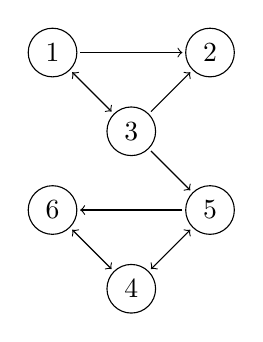
\begin{tikzpicture}
            \draw (0,0) node[circle,draw]{3};
            \draw (-1,1) node[circle,draw]{1};
            \draw (1,1) node[circle,draw]{2};
            \draw (-1,-1) node[circle,draw]{6};
            \draw (1,-1) node[circle,draw]{5};
            \draw (0,-2) node[circle,draw]{4};
        %
            \draw[<->] (-0.25,0.25) -- (-0.75,0.75);
            \draw[->] (-0.65,1) -- (0.65,1);
            \draw[->] (0.25,0.25) -- (0.75,0.75);
            \draw[->] (0.25,-0.25) -- (0.75,-0.75);
            \draw[->] (0.65,-1) -- (-0.65,-1);
            \draw[<->] (-0.75,-1.25) -- (-.25,-1.75);
            \draw[<->] (0.75,-1.25) -- (0.25,-1.75);
        \end{tikzpicture}
    \end{center}
        \caption{Sample graph of a web with six pages.}
        \label{fig:example_graph}
\end{figure}

We will first define some notation in the PageRank algorithm:
\begin{itemize}
    \item $|P_i|$ is the number of outlinks from page $P_i$
    \item $H$ is the {\it hyperlink} matrix defined as 
        \[ H_{ij} = \left\{ \begin{array}{cl} \frac{1}{|P_j|}, & \text{if there is a link
            from node $j$ to node $i$} \\ 0, & \text{otherwise} \end{array} \right. \]
        where the ``$i$'' and ``$j$'' are the row and column indices respectively.  
    \item $\bx$ is a vector that contains all of the PageRanks for the individual pages.
\end{itemize}

The PageRank algorithm works as follows:
\begin{enumerate}
    \item Initialize the page ranks to all be equal. This means that our initial
        assumption is that all pages are of equal rank.  In the case of Figure
        \ref{fig:example_graph} we would take $\bx_0$ to be 
        \[ \bx_0 = \begin{pmatrix} 1/6 \\ 1/6 \\ 1/6 \\ 1/6 \\ 1/6 \\ 1/6 \end{pmatrix}. \]
    \item Build the hyperlink matrix.  \\ As an example we'll consider node 3 in Figure
        \ref{fig:example_graph}.  There are three outlinks from node 3 (to nodes 1, 2, and
        5).  Hence $H_{13}=1/3$, $H_{23} = 1/3$, and $H_{53} = 1/3$ and the partially
        complete hyperlink matrix is
        \[ H = \begin{pmatrix} 
                - & - & 1/3 & - & - & - \\
                - & - & 1/3 & - & - & - \\
                - & - & 0   & - & - & - \\
                - & - & 0   & - & - & - \\
                - & - & 1/3 & - & - & - \\
                - & - & 0   & - & - & - 
            \end{pmatrix} \]
    \item The difference equation $\bx_{n+1} = H \bx_n$ is used to iteratively refine the
        estimates of the page ranks.  You can view the iterations as a person visiting a
        page and then following a link at random, then following a random link on the next
        page, and the next, and the next, etc.  Hence we see
        that the iterations evolve exactly as expected for a difference equation.
        \begin{center}
            \begin{tabular}{|c|c|}
                \hline
                Iteration & New Page Rank Estimation \\ \hline \hline
                0 & $\bx_0$ \\
                1 & $\bx_1 = H \bx_0$ \\
                2 & $\bx_2 = H \bx_1 = H^2 \bx_0$ \\
                3 & $\bx_3 = H \bx_2 = H^3 \bx_0$ \\
                4 & $\bx_4 = H \bx_3 = H^4 \bx_0$ \\
                \vdots & \qquad \vdots \\
                $k$ & $\bx_k = H^k \bx_0$ \\ \hline
            \end{tabular}
        \end{center}
    \item When a steady state is reached we sort the resulting vector $\bx_k$ to give the
        page rank. The node (web page) with the highest rank will be the top search
        result, the second highest rank will be the second search result, and so on.
\end{enumerate}

It doesn't take much to see that this process can be very time consuming.  Think about
your typical web search with hundreds of thousands of hits; that makes a square matrix $H$
that has a size of hundreds of thousands of entries by hundreds of thousands of entries!
The matrix multiplications alone would take many minutes (or possibly many hours) for
every search! \dots but Brin and Page were pretty smart dudes!!


We now state a few theorems and definitions that will help us simplify the iterative
PageRank process.
\begin{thm}\label{thm:eigen_expand}
    If $A$ is an $n \times n$ matrix with $n$ linearly independent eigenvectors $\bv_1,
    \bv_2, \bv_3,$ $\ldots, \bv_n$ and associated eigenvalues $\lambda_1, \lambda_2,
    \lambda_3, \ldots, \lambda_n$ then for any initial vector $\bx \in \mathbb{R}^n$ we
    can write $A^k \bx$ as
    \[ A^k \bx = c_1 \lambda_1^k \bv_1 + c_2 \lambda_2^k \bv_2 + c_3 \lambda_3^k \bv_3 +
        \cdots c_n \lambda_n^k \bv_n \]
    where $c_1, c_2, c_3, \ldots, c_n$ are the constants found by expressing $\bx$ as a
    linear combination of the eigenvectors. \\Note: We can assume that the eigenvalues are ordered
    such that $\lambda_1 \ge \lambda_2 \ge \lambda_3 \ge \cdots \ge \lambda_n$.
\end{thm}
\begin{proof}
    (Prove the preceding theorem)
\end{proof}

\begin{definition}
    A {\bf probability vector} is a vector with entries on the interval $[0,1]$ that add up to 1. 
\end{definition}
\begin{definition}
    A {\bf stochastic matrix} is a square matrix whose columns are probability vectors.
\end{definition}

\begin{thm} \label{thm:largest_ev_stochastic}
    If $A$ is a stochastic $n \times n$ matrix then $A$ will have $n$ linearly independent
    eigenvectors.  Furthermore, the largest eigenvalue of a stochastic matrix will
    \underline{always} be $\lambda_1 = 1$ and the smallest eigenvalue  will always be
    nonnegative: $0 \le \lambda_n < 1$.
\end{thm}

Some of the following tasks will ask you to {\it prove} a statement or a theorem.  This
means to clearly write all of the logical and mathematical reasons why the statement is
true. Your proof should be absolutely crystal clear to anyone with a similar mathematical
background \dots if you are in doubt then have a peer from a different group read your
proof to you \underline{out loud}.

\begin{problem}
    Finish writing the hyperlink matrix $H$ from Figure \ref{fig:example_graph}.
\end{problem}

\begin{problem}
    Write MATLAB code to implement the iterative process defined previously. Make a plot
    that shows how the rank evolves over the iterations.
\end{problem}


\begin{problem}
    What must be true about a collection of $n$ pages such that an $n\times n$
        hyperlink matrix $H$ is a stochastic matrix.
\end{problem}

The statement of the next theorem is incomplete, but the proof is given to you.  Fill in
the blank in the statement of the theorem and provide a few sentences supporting your
answer.
\begin{thm}\label{thm:steady}
    If $A$ is an $n \times n$ stochastic matrix and $\bx_0$ is some initial vector
    for the difference equation $\bx_{n+1} = A \bx_n$, then the steady state
    vector is
    \[ \bx_{equilib} = \lim_{k \to\infty} A^k \bx_0 = \underline{\hspace{1in}}. \]
\end{thm}
\begin{proof}
    First note that $A$ is an $n \times n$ stochastic matrix so from Theorem
    \ref{thm:largest_ev_stochastic} we know that there are $n$ linearly
    independent eigenvectors.  We can then substitute
    the eigenvalues from Theorem \ref{thm:largest_ev_stochastic} in Theorem
    \ref{thm:eigen_expand}. Noting that if $0<\lambda_j<1$ we have $\lim_{k \to
    \infty} \lambda_j^k = 0$ the result follows immediately.
\end{proof}
\begin{problem}
    Discuss how Theorem \ref{thm:steady} greatly simplifies the PageRank iterative process
    described previously.  In other words: there is no reason to iterate at all.  Instead,
    just find \underline{\hspace{1in}}.
\end{problem}
\begin{problem}
\item Now use the previous two problems to find the resulting PageRank vector from the web in Figure
    \ref{fig:example_graph}?  Be sure to rank the pages in order of importance.
    Compare your answer to the one that you got in problem 2.
\end{problem}


\begin{problem}
    Consider the web in Figure \ref{fig:graph2}.
        \begin{enumerate}
            \item[(a)] Write the $H$ matrix and find the initial state $\bx_0$, 
            \item[(b)] Find
                steady state PageRank vector using the two different methods described:
                one using the iterative difference equation and the other using Theorem
                \ref{thm:steady} and the dominant eigenvector.
            \item[(c)] Rank the pages in order of importance.
        \end{enumerate}
\end{problem}
\begin{figure}[ht!]
    \begin{center}
        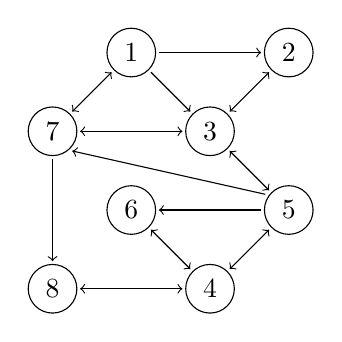
\begin{tikzpicture}
            \draw (0,0) node[circle,draw]{3};
            \draw (-1,1) node[circle,draw]{1};
            \draw (1,1) node[circle,draw]{2};
            \draw (-1,-1) node[circle,draw]{6};
            \draw (1,-1) node[circle,draw]{5};
            \draw (0,-2) node[circle,draw]{4};
            \draw (-2,0) node[circle,draw]{7};
            \draw (-2,-2) node[circle,draw]{8};
        %
            \draw[<-] (-0.25,0.25) -- (-0.75,0.75);
            \draw[->] (-0.65,1) -- (0.65,1);
            \draw[<->] (0.25,0.25) -- (0.75,0.75);
            \draw[<->] (0.25,-0.25) -- (0.75,-0.75);
            \draw[->] (0.65,-1) -- (-0.65,-1);
            \draw[<->] (-0.75,-1.25) -- (-.25,-1.75);
            \draw[<->] (0.75,-1.25) -- (0.25,-1.75);
            \draw[<->] (-1.75,0.25) -- (-1.25,0.75);
            \draw[<->] (-1.65,0) -- (-0.35,0);
            \draw[<-] (-1.75,-0.25) -- (0.7,-0.8);
            \draw[->] (-2,-0.35) -- (-2,-1.65);
            \draw[<->] (-1.65,-2) -- (-0.35,-2);
        \end{tikzpicture}
    \end{center}
    \caption{Graph of a web with eight pages.}
    \label{fig:graph2}
\end{figure}


\begin{problem}
    One thing that we didn't consider in this version of the Google Page Rank algorithm is
    the random behavior of humans.  One, admittedly slightly naive, modification that we
    can make to the present algorithm is to assume that the person surfing the web will
    randomly jump to any other page in the web at any time.  For example, if someone is on
    page 1 in Figure \ref{fig:graph2} then they could randomly jump to any page 2 - 8.
    They also have links to pages 2, 3, and 7.  That is a total of 10 possible next steps
    for the web surfer.  There is a $2/10$ chance of heading to page 2.  One of those is
    following the link from page 1 to page 2 and the other is a random jump to page 2
    without following the link.  Similarly, there is a $2/10$ chance of
    heading to page 3, $2/10$ chance of heading to page 7, and a $1/10$ chance of randomly
    heading to any other page.

    Implement this new algorithm, called the {\it random surfer algorithm}, on the web in
    Figure \ref{fig:graph2}.  Compare your ranking to the non-random surfer results from
    the previous problem.
\end{problem}


\newpage\section{Additional Exercises}
\begin{problem}
    Let $\bv_1 = \begin{pmatrix} 5\\1\end{pmatrix}$ and $\bv_2 =
    \begin{pmatrix}1\\-1\end{pmatrix}$ be eigenvectors of a matrix $A$ corresponding to
    eigenvalues $\lambda_1 = -2$ and $\lambda_2 = 5$ respectively.  Compute $A(\bv_1 +
    \bv_2)$ and $A(3\bv_1)$.
\end{problem}
\hint{
    Recall that if $A$ has eigenvector $\bv$ and eigenvalue $\lambda$ then $A\bv = \lambda
    \bv$.
}

\begin{problem}
    Long ago, in a galaxy far, far away \dots there are two cell-phone companies serving a
    town: the Evil Empire and the Rebel Alliance. The Evil Empire has terrible service, so
    each week 25\% of their customers switch to the Rebel Alliance and 2\% give up their
    cell phone service entirely. The Rebel Alliance loses only 5\% of their customers to
    the Evil Empire every week due to the advertising.  If there are currently 100
    customers in the Evil Empire and 75 customers in the Rebel Alliance, what is the
    long-term enrollment in the two plans?

    Write a system of difference equations and use the ideas of eigenvalues and
    eigenvectors to discuss the long-term behavior of the system.
\end{problem}
\solution{
    \begin{flalign*}
        \begin{pmatrix} E_{n+1} \\ R_{n+1} \end{pmatrix} &=\begin{pmatrix} E_n \\ R_n
        \end{pmatrix} +  \begin{pmatrix} -0.27 & 0.05 \\ 0.25 & -0.05  \end{pmatrix}
        \begin{pmatrix} E_n \\ R_n \end{pmatrix} \\
        \implies 
        \begin{pmatrix} E_{n+1} \\ R_{n+1} \end{pmatrix} &=\begin{pmatrix} 0.73 & 0.05 \\
            0.25 & 0.95  \end{pmatrix}
        \begin{pmatrix} E_n \\ R_n \end{pmatrix} \\
    \end{flalign*}
    The eigenvalues of the coefficient matrix are $\lambda_1 \approx 0.68$ and $\lambda_2
    \approx 0.9968$.  Since both of these are less than 1 we know that the eventual
    behavior is that both companies will lose their customers although the Evil Empire
    will lose at a faster rate.
}


\begin{problem}
    Find a $2 \times 2$ matrix such that $\bv_1 = \begin{pmatrix}-2\\-3\end{pmatrix}$ and
    $\bv_2=\begin{pmatrix}0\\1\end{pmatrix}$ are eigenvectors of $A$ with eigenvalues $5$
    and $-1$ respectively.
\end{problem}
\hint{
    Recall that if $A$ has a full collection of eigenvalues and eigenvectors then $A =
    PDP^{-1}$.  Build the matrices $P$ and $D$ and you can build $A$.
}


\begin{problem}
    The Cayley-Hamilton Theorem states that a matrix will satisfy its own characteristic
    polynomial.  Recall that for a matrix $A$ the characteristic polynomial is $p(\lambda)
    = \det(A - \lambda I)$ and to find the eigenvalues $\lambda$ we solve the equation
    $p(\lambda) = 0$.  The Cayley-Hamilton Theorem states that $p(A) = 0$ where the ``0''
    here means that zero matrix.  
    \begin{enumerate}
        \item[(a)] Let $A = \begin{pmatrix} -4 & 4 \\ -4 & -3 \end{pmatrix}$.  Use the
            Cayley-Hamilton Theorem to find a quadratic polynomial $p$ such that $p(A) =
            0$.
        \item[(b)] For a matrix $A$ assume that $(A - 2I)(A+3I) = 0$.  There are
            infinitely many matrices $A$ for which this algebraic equation is true.  What
            characteristics do all of the matrices have?
    \end{enumerate}
\end{problem}
\hint{
    \begin{enumerate}
        \item[(a)] Find the characteristic polynomial for $A$.
        \item[(b)] The expression $(A-2I)(A+3I)=0$ implicitly gives the characteristic
            polynomial for $A$ and hence you can find the eigenvalues.  
    \end{enumerate}
}


\begin{thm}\label{thm:eigenstructure1}
    Let $A$ be an $n\times n$ matrix.  For every positive integer $k$, $A^k$ will have the
    same eigenvectors as $A$.
\end{thm}
\begin{problem}
    \begin{enumerate}
        \item[(a)] Prove Theorem \ref{thm:eigenstructure1}.
        \item[(b)] If $\bv$ is an eigenvector of the matrix $A$ with eigenvalue $\lambda$
            then what is the eigenvalue of $\bv$ associated with $A^k$ for some positive
            integer $k$?
    \end{enumerate}
\end{problem}


\begin{thm}\label{thm:eigenstructure2}
    Let $A$ be an $n\times n$ matrix.  For every real number $c$ the matrices $(A + cI)$ and
    $cA$ will have the same eigenvectors as $A$.
\end{thm}
\begin{problem}
    \begin{enumerate}
        \item[(a)] Prove Theorem \ref{thm:eigenstructure2}.
        \item[(b)] If $\bv$ is an eigenvector of the matrix $A$ with eigenvalue $\lambda$
            then what are the eigenvalues of $\bv$ associated with $(A+cI)$ and $cA$ for some
            integer $c$?
    \end{enumerate}
\end{problem}


% \begin{thm}\label{thm:eigenstructure3}
%     Let $A$ be an $n\times n$ invertible matrix.  The matrix $A^{-1}$ has the same
%     eigenvectors as $A$.
% \end{thm}
% \begin{problem}
%     \begin{enumerate}
%         \item[(a)] Prove Theorem \ref{thm:eigenstructure3}.
%         \item[(b)] If $\bv$ is an eigenvector of the matrix $A$ with eigenvalue $\lambda
%             \neq 0$
%             then what is the eigenvalue of $\bv$ associated with $A^{-1}$?
%     \end{enumerate}
% \end{problem}



\begin{problem}
    Is $\lambda = 2$ an eigenvalue of $\begin{pmatrix}3&2\\1&2\end{pmatrix}$?  Why or why
    not?
\end{problem}


\begin{problem}
    Suppose that the vector {\color{blue} $\bx$} is a real-valued eigenvector of the matrix $M$ and that
    the entries of $M$ are also real valued.
    \begin{enumerate}
        \item[(a)] Considering the vectors plotted below, what could be the result of the
            product $M\bx$?  Circle all that apply.
            \begin{center}
                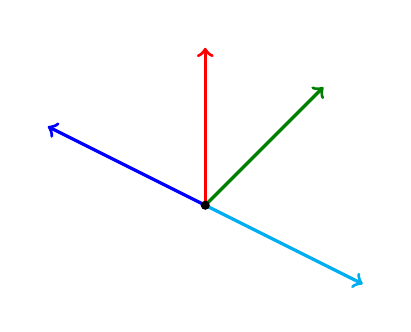
\begin{tikzpicture}
                    \draw[very thick, blue, ->] (0,0) -- (-2,1) node[anchor=south east]{$\bx$};
                    \draw[very thick, red, ->] (0,0) -- (0,2) node[anchor=south]{$\bu$};
                    \draw[very thick, green!50!black, ->] (0,0) -- (1.5,1.5) node[anchor=south west]{$\bv$};
                    \draw[very thick, cyan, ->] (0,0) -- (2,-1) node[anchor=north west]{$\bw$};
                    \draw[fill=black] (0,0) circle(0.05cm) node[anchor=north east]{$\bo$};
                \end{tikzpicture}
            \end{center}
            \begin{itemize}
                \item[(i)] $M{\color{blue} \bx}$ could be {\color{red} $\bu$}.
                \item[(ii)] $M{\color{blue} \bx}$ could be {\color{green!50!black} $\bv$}.
                \item[(iii)] $M{\color{blue} \bx}$ could be {\color{cyan} $\bw$}.
                \item[(iv)] $M{\color{blue} \bx}$ could be {\color{black} $\bo$}.
                \item[(v)] $M{\color{blue} \bx}$ could be {\color{blue} $\bx$}.
                \item[(vi)] None of the above
            \end{itemize}
        \item[(b)] Explain your reasoning for your choice(s) in part (a).
    \end{enumerate}
\end{problem}
